\chapter{\acl{sota}}
\label{chapter:sota}

\section{Datasets}
\label{section:sota:datasets}

Training an autonomous vehicle to be capable of driving himself is a complex challenge with multiple parts and problems to be solve: recognizing other users of the road (persons, vehicles, cyclists); understanding traffic signs; track and estimate the movement of the road users; plan the path; accurate modelling of the environment; among many others. To both train neural networks and other genetic algorithms, but also to intensevely test systems and other software, huge amounts of data are required.

To accelerate this progress, a collaborative effort is being made to release datasets online for free public usage under permissive licenses. This datasets vary in their objective, sensory data available, conditions whose data has been acquired, driving conditions and format on which they are provided, among other aspects. 

Despite this work having no intentions to study autonomous driving, the algorithms developed for calibration, sensor fusion and computing the correspondence between objects of interest in image and point cloud are not meant to be particular applied on datasets with interference. Therefore, using public available datasets not only allow the development of those algorithms before experimental data can be gathered, but also wides the aplicability of such work, without losing their applicability to the particular situation of \ac{lidar} interference.

During the months when this research work was carried, several new datasets were made available online, such as nuScenes~\cite{nuScenes2019} and Waymo~\cite{Waymo}. Since no new contribute was expectd from their usage besides the ones already provided by the datasets already in use on this research, no further reseach on them was carried. 

For the purposes of this research, several datasets were considered and tested. On the next sections, a brief summary is given about the ones that have sensory data from camera and \ac{lidar}. Those were the candidates to be used on this work.

\subsection{Ford Campus \ac{lidar} dataset}
Gathered in 2009, in Michigan, the Ford Campus \ac{lidar} dataset contains camera, \ac{lidar}, \ac{imu} and \ac{gps} data. The dataset consists of two test scenarios, one inside the Ford Research campus and another on downtown Dearborn. A small subset of the former test scenario is also provided.

The data is provided in raw format, accompanied by log files with timestamps, \ac{gps} and \ac{lcm}\footnote{For more information on \acf{lcm} protocol for estimating delays between the registered of sensory data on master-slave systems, see~\cite{VelodyneHDL64}.} logs with all raw data. The images from an omnidirectional camera, a Point Grey Ladybug3, are stored on \ac{ppm}; \ac{lidar} data from a Velodyne HDL-64E on \ac{pcap} format, from the \ac{tcp} connection socket; two Riegl LMS-Q120 \acp{lidar} also provide more information on the scan.

The data is rectified and synced under \ac{matlab} \textit{.mat} files. Along with the raw data and synced and rectified \textit{.mat} files, source code is also provided for parsing the raw data, visualizing the \ac{lcm} logs and pre-processed data on \ac{matlab}. A C and \ac{opengl} software that can render textured point clouds is also available.

The modified Ford F-250 pickup truck, which can be seen on figure~\ref{fig:sota:ford_sensors}, uses 3 sensors for navigation~\cite{Pandey2011}: one 3D \ac{lidar}, Velodyne HDL-64E \ac{lidar}~\cite{VelodyneHDL64}; one camera: Point Grey Ladybug3 omnidirectional camera; and two 2D \acp{lidar}: Riegl LMS-Q120 lidar. More details about the sensors, their relative positioning and data formats and files can be found~\cite{Pandey2011}.

\begin{figure}
	\centering
	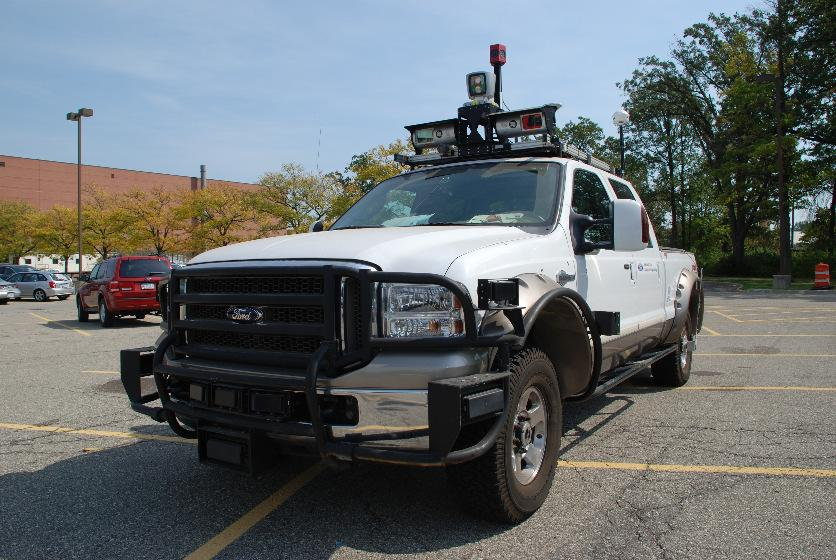
\includegraphics[width=0.5\textwidth]{img/sensor_fusion/ford_sensors.jpg}
	\caption{Ford 250 pickup equipped with the sensors descibed in the previous paragraphs. On the top, the Ladybug omnidirectional camera, on the back the \ac{imu} and \ac{gps} unit. }
	\label{fig:sota:ford_sensors}
\end{figure}


\subsection{\ac{kitti}}
A well known dataset for researchers of computer vision, autonomous driving and \ac{ml}, \ac{kitti} was recorded in 2011 and released for the public in 2013. This dataset contains various driving scenarios: suburban, highways, residential and campus areas; with trucks, cars, cyclists and persons. Alongside with data for testing, calibration measures are provided for all sensors.

The test car, a Volkswagen Passat is equipped with two stereo pairs, one with color and other with gray cameras, a \ac{lidar}, an \ac{imu} and a\ac{gps} sensor. Data from all four cameras is stored on \ac{png} format, \ac{lidar} measurements as a binary float matrix, \ac{gps} and {imu} data textually. Additionally to the raw data, logs containing the timestamps and the transforms between the sensors are also provided. Labeled data is also available for some test scenarios on \ac{xml} files.

Along with the data and calibration parameters, several tools written in C++ or \ac{matlab} are also provided. The dataset offers two types of data categories: (1) unsynced and unrectified data or (2) synced and rectified data. 

The sensory apparatus contains 2 PointGray Flea2 greyscale and color cameras, a Velodyne HDL-64E \ac{lidar}~\cite{VelodyneHDL64}, among others less relevant sensors~\cite{Geiger2013a}.

\begin{figure}
	\centering
	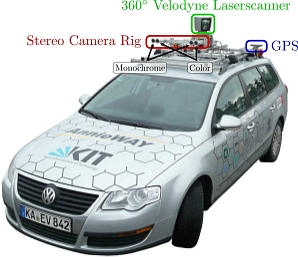
\includegraphics[width=0.5\textwidth]{img/sensor_fusion/passat_sensors.jpg}
	\caption{Volkswagen Passat equipped with the sensors descibed in the previous paragraphs, for the \ac{kitti} dataset. On the top, the Velodyne \ac{lidar} and below the 2 stereo pairs (color and grey). On the back, the \ac{imu} and {gps} systems are present.}
	\label{fig:sota:kitti_sensors}
\end{figure}


\subsection{Udacity Self-Driving Car Nanodegree Dataset}
Available publicly is also the data from Udacity online course on self-driving car. This dataset dates back to 2016 and was gathered with the intent to develop a level 4 autonomy vehicle, containing much more data diversity than the previous two. The data available contains images from 3 color cameras, a \ac{lidar} data, \ac{imu} and \ac{gps}, among other sensory data, such as speed, braking, etc.

Their data is not available in raw format, only structured in \ac{ros} \textit{.bag} files. Some tools for visualizing and interacting with their data are provided for \ac{ros}~\cite{udacity}. 

Not much information is publicaly available, and the dataset contains to calibration data between its sensors.

\subsection{Summary}
Table~\ref{tab:sota:datasets_comparison} summarizes all the relevant data from the datasets~\cite{udacity, Pandey2011, Geiger2013a}. We can see that there are few differences between the relevant types of data gather but major differences can be seen on the format provided. While \ac{kitti} not only provides the largest dataset in quantity, but also provides rectified and synced data. For the purposes of this research, there is no interest in testing syncing and rectification methods, which penalizes Ford dataset. 

While Udacity dataset is the newest and provides direct out-off-the-shelf integration with \ac{ros}, that type of integration can also be achieved for \ac{kitti} by using other tools, such as \textit{kitti2bag}~\cite{TomasKrejci}. 
	
\begin{table}[H]
	 \rowcolors{4}{gray!10}{white}
	 \renewcommand{\arraystretch}{1.2}
	 \centering
	\begin{tabular}{llccc}
																& & \multicolumn{3}{c}{Datasets} \\ \cline{3-5}
																& & Ford Campus  & \acs{kitti} & Udacity \\ \midrule
																& \ac{lidar}	& \checkmark  & \checkmark & \checkmark \\ 
																& Color Camera & \checkmark   &  \checkmark  &  \checkmark  \\
																& Grey Cameras &  &  \checkmark  &  \\
																& Stereo Camera &  &  \checkmark  &  \checkmark  \\
																& Omnidirectional Camera &  \checkmark  &  &  \\
																& \acs{imu} &  \checkmark  &  \checkmark  &  \checkmark  \\
																& \acs{gps} &  \checkmark  &  \checkmark  &  \checkmark  \\
		\rowcolor{white}\multirow{-8}{*}{Data Types} 														& Other data relevant to autonomous driving & & & \checkmark \\
		\multirow{5}{*}{Formats and Tools} & Raw data available &  \checkmark  &  \checkmark  &  \\
																			 & Data parsing tools &  \checkmark  &\checkmark    &  \checkmark  \\
																			 & Rectified data & & \checkmark  & \\
																			 & Synced data &  & \checkmark   &  \checkmark  \\ 
																			 & Calibration parameters & \checkmark  & \checkmark  & \checkmark  \\
		\multicolumn{2}{l}{Raw data for calibration} & & \checkmark & \\
		\multicolumn{2}{l}{\ac{ros} data compatibility} &  &  \checkmark\footnotemark &  \checkmark  \\
		\bottomrule
	\end{tabular}
\caption{Comparison between the datasets more appropriated to this thesis objectives}
\label{tab:sota:datasets_comparison}
\end{table}
\footnotetext{Requires the usage of an external tool \textit{kitti2bag}~\cite{TomasKrejci}} 

At the time this research began, Udacity and \ac{kitti} data sets are the most appealing to be used. Prioritizing ease of use, Udacity data set trumps over \ac{kitti}, since \ac{ros} will be a tool usage on this research as well.


	
